\section{System Overview (75 pts)\label{sec:1}}

    \begin{figure}
        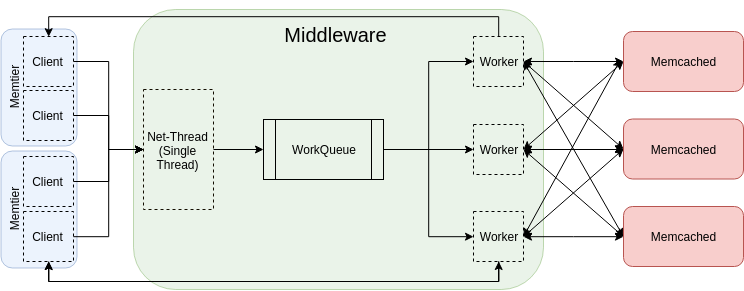
\includegraphics[width=0.8\linewidth]{graphics/system-request-flow.png}
        \caption{Basic flow of information in the system. Each box with a dashed border indicates a thread on the
                 respective system which are colour coded into 3 categories, blue for \cli, green for \mw{} and red for
                 \srv. Arrows denote the order of flow of information.\label{fig:request-overview}}
    \end{figure}

    The basic flow of requests through the system is visualized in figure \ref{fig:request-overview}. A basic lifetime
    of a request begins in a thread on a middleware, is received by the Net-Thread and upon receiving a complete packet
    it is stored in the WorkQueue. This queue is shared for any threads in the middleware and they compete for each
    individual element. The moment a Worker receives the request it processes it locally, checks the type and first
    sends the request to either one connected memcached (non-sharded GET) or all connected memcached instances connected
    (sharded GET and SET). Upon receiving replies from memcached there are also checks for what was received and sanity
    checks included (e.g. receiving a SET reply for a GET reply is clearly an ERROR) before sending back a constructed
    reply directly from the Worker to the Client given enough replies have been received. As such the Middleware
    receives only via the Net-Thread and only sends only via the Worker when communicating with memtier instances.
    Communication between memcached is synchronously designed, each Worker connecting to all available memcached
    instances.

    \subsubsection{System Component Overview}
        For network communication Java NIO is used for all connections. The Net-Thread uses a \tw{ServerSocketChannel}
        whereas worker threads employ for each connection with memcached an instance-private \tw{SocketChannel}, all
        connections configured to be non-blocking. With the use of Java NIO \tw{Channel}s writes are expected to be
        perform more ideal in distribution from the middleware to either memcached or memtier. To manage connections the
        Net-Thread employs a single \tw{Selector} which handles memtier connections, each worker thread two\textemdash
        one to manage all memcached connections and another to interact with memtier using referenced \tw{SelectionKey}s
        from the Net-Thread's Selector. To allow handling of multiple requests the Net-Thread spawns a fixed amount of
        worker threads once at the start, all attached to an \tw{ExecutorService} and upon finishing return gathered
        thread statistics. This is achieved by worker threads implementing the \tw{Callable} interface. The gathered
        statistics are to be saved by the net-thread for each finished worker before termination. Termination can be
        achieved by sending the middleware a \tw{SIGTERM} signal; a shutdown hook is installed right after the
        middleware is instantiated by the given wrapper class.\newline
        For the WorkQueue depicted an \tw{ArrayBlockingQueue} is used, meaning blocking behaviour can be expected for
        the Net-Thread if the queue fills up with requests and blocking behaviour for workers should not enough requests
        exist. As such the only producer is the Net-Thread and the only consumers worker threads. The content of the
        WorkQueue are \tw{WorkUnit}s which are interpreted requests/replies and designed to be more programmer friendly
        than simple \tw{byte[]}-arrays at the expense of more garbage collection. These WorkUnits are the result of
        successfully receiving data from either party and the product of a \tw{PacketParser}, used by connections of the
        Net-Thread and worker threads. It is designed in a stateful approach and as such each connection has a logically
        private instance of a PacketParser attached to it. This binding is done after the first successful registration
        of new connections.

    \subsubsection{Request Handling}
        Before any requests are processed by the middleware any incoming memtier connections must be first
        \tw{accept()}-ed by the Net-Thread and registered in the attached Selector. Once done the PacketParser is called
        each time the OS notifies of new data being available on a registered SelectionKey. The PacketParser is designed
        to read data from a socket into a directly allocated \tw{ByteBuffer} (size = \SI{8192}{\byte}), generate a
        timestamp for the call to read data from the socket, receive data from the socket, parse the received data and
        extract at most a single request/reply, compact the ByteBuffer and store the result on success. This process is
        repeated as long as a request is stored (this will all in all return a \tw{List}) and as such follows a greedy
        approach. The design aims to fully exhaust the data received from a single client before parsing new data. This
        would be troublesome in the general case of long streams but this is not expected and aims to allow quicker
        handling of single requests once they get actively processed. In the process of extracting data three basic
        steps follow; read the current stream of Bytes linearly until \tw{"\textbackslash r\textbackslash n"} is
        encountered, extract the data and match it Byte-by-Byte to a list of supported headers and extract type-specific
        header fields as per memcached documentation, and lastly either return the result as no body is expected or try
        to get the rest of the body.  The body is read in a single command as is therefore likely to need multiple
        repetitions as MTUs are limited to \SI{1500}{\byte} but the body size being \SI{4096}{\byte}. As such internal
        state is kept over rounds as to what part of a packet is currently expected to be processed. Once enough data is
        buffered the data is then copied and the result returned. As previously noted this result is a \tw{WorkUnit}. It
        holds next to the received header and body (as \tw{byte[]}) also fields for the type, type-specific fields (such
        as the list of keys for GET requests), the SelectionKey from which it was received and also a timestamp-object
        which keeps track on statistics when a packet was received (the iteration where the header is parsed is stored),
        enqueued into the WorkQueue, dequeued from it, when it was ready to be sent to memcached, when all replies were
        received for it from memcached and finally when the reply was sent back to memtier.\newline
        The PacketParser returns once all data was consumed and returns a list of received packets. These are then
        stored to the WorkQueue for worker threads to process.

        Processing WorkUnits on a worker follows the outline of dequeueing an element, checking its type, sending the
        request to either one (non-sharded GET) or all/some connected memcached servers (sharded multi-key GET or SET),
        waiting for the appropriate amount of replies, doing some local processing of the replies, sending it to the
        WorkUnit's attached SelectionKey and then dequeue another element, thus restarting the loop. Upon dequeueing the
        element is checked to be of type GET, SET, an invalid packet or anything else (the latter two resulting in
        logged messages). For SET requests the worker thread prepares for each memcached-instance connected to a new
        ByteBuffer with a copy of the request and sends it to all memcached servers. It waits for each server to reply
        with 3 messages and verifies the content to be only STORED. On a failure an error message is returned, on a
        match any of the three requests chosen and sent back to the recipient by dereferencing the associated
        SocketChannel with the original WorkUnit by use of ByteBuffer. GET requests are prepared with load-balancing
        schemes (described in thorough detail later) depending on enabling or disabling sharding. The amount of keys in
        each GET (making it essentially a so called \emph{MultiGET}) is irrelevant to the code path followed for
        sharding. For the non-sharded case a single packet (a ByteBuffer in code) is created, the size remembered for
        load-balancing purposes and mapped to the server with the smallest load. For the sharded case mappings of
        packets to servers in the degree of distributed load are generated. Skewed loads result in the degenerated case
        of a non-sharded multi-GET, good cases in a fair distribution of requests to servers (logically, they have not
        yet been sent, only prepared).  After the packets are created and mapped to servers an expectation of replies is
        set for each memcached instance and the routine referenced in the distribution of SET requests is called. It is
        universal enough to also deal with misses and stops listening to the memcached instance once an ``END'' is
        received and internal state updated. After receiving all necessary replies sanity checks are again made,
        received ``VALUE'' requests serialized and an ``END'' packet appended to the collection of packets before a
        ByteBuffer is created from the replies and then sent to the respective memtier instance. In all cases where
        replies are received from memcached the associated PacketParser is used to read the received data and resulting
        WorkUnits stored in a result list. These WorkUnits are only processed locally to infer the validity of the
        reply and build one for memcached, nothing more.

    \subsubsection{System Instrumentation}
        For the following events in the system performance benchmarking results are generated: In the PacketParser on
        the relating call when a header is correctly parsed (\textrightarrow{} timestamp for package arrived in the
        system, stored in the respective WorkUnit), on an enqueue and dequeue to the WorkQueue (\textrightarrow{} the
        current queue size is logged after the operation completed successfully, the only statistic on the Queue;
        additionally in both cases the WorkUnit gets the timestamp logged for the respective event) and at the following
        points in the worker thread. The aforementioned dequeue also generates packet-type specific metrics. For all
        valid types (SET, GET and multi-GET) the count of observed elements is incremented and the time on the queue
        logged. GETs of multiple keys also log the amount of keys. For invalid packets a counter is incremented. Before
        communication with memcached occurs but after the keys have already been mapped for servers and created a
        timestamp is stored in the WorkUnit. In case of an unexpected amount of GET replies the number of missing keys
        is logged for GET requests disregarding their size. It is still possible to infer whether a single-sized key was
        the reason or a multi-key GET. Another timestamp is generated after receiving and having processed all
        request-related replies as well. In addition to this timestamp the communication with memcached and packet
        processing is logged for the respective request type. A last timestamp is stored the moment the reply has been
        successfully written to memcached's SocketChannel. This again also incurs and store of the total duration the
        WorkItem has been in the system and simulates an RTT through the system in addition to generating a statistic
        used for creating histograms. Lastly at termination of the each worker thread the observed load distribution is
        remembered. All datapoints captured by a worker are upon termination accumulated and averaged (where applicable)
        in relation to the percentage of requests they served.\newline
        Timestamps on WorkItems are used to populate the aforementioned type-specific request metrics. All metrics
        mentioned that are not timestamps are accumulated in 1 second windows and in all cases but the load distribution
        and counters for requests / cache misses are averaged by the number of observed datapoints. This averaging is a
        simple arithmetic mean. The metrics on cache misses and request counts are simple counts and not averaged. The
        load distribution is continuously updated but returns an overall view at the end of the lifetime of the thread.

        To start logging a common timestamp is set once the first packet has been fully parsed and ready to be dequeued.
        A final timestamp is set in the Net-Thread after all worker threads have finished execution.

    % Internally the \tw{PacketParser} has the notion of a header and body. Headers are matched on a new packet by
    % searching for the String \tw{"\textbackslash r\textbackslash n"} and then the extracted header is matched
    % byte-by-byte to all possible headers. A partially constructed \tw{WorkUnit} (i.e. parsed packet) is created and the
    % timestamp from the last socket read used as the starting timestamp for calculations how long packets were in the
    % system. The byte-by-byte matching sets an upcoming expectation on what the type must be. For GET requests the header
    % is again evaluated and any keys extracted which are available (GET with a single key and GET with multiple keys are
    % parsed exactly the same). No body exists for it and as such the \tw{PacketParser} can return it quickly. For a SET
    % request a body is expected. The next \SI[number-math-rm = \mathnormal, parse-numbers = false]{n+2}{\mybyte} (with
    % $n$ = 4096 for the experiments, smaller packets are also possible to be parsed) are buffered in and then read in one
    % contiguous allocation. Sanity checks are performed and the last two Bytes verified to also be \tw{"\textbackslash
    % r\textbackslash n"}. On a missmatch the line is consumed until such a sequence is encountered and the incorrectly
    % formatted packet made available for consumption where memcached is expected to return an ERROR.  For the replies to
    % SET and GET (STORED and VALUE) analogous approaches are done depending on the existence of respective
    % fields.\newline

    % Before Workers can get active, a request must be put onto the WorkQueue (implemented using an
    % \tw{ArrayBlockingQueue}). The WorkQueue is solely populated by the Net-Thread which uses a Java NIO
    % \tw{ServerSocketChannel} to handle incoming connections by memtier clients. It calls the \tw{accept()} method to
    % accept and register new clients and additionally instantiates and binds a stateful \tw{PacketParser} on each
    % client's \tw{SelectionKey} which uses a directly allocated \tw{ByteBuffer} of \SI{8192}{\mybyte} to locally buffer
    % packets. The buffer's size is large enough to handle any packet sent by memtier (as packets are limited to a maximum
    % size of \SI{4132}{\mybyte}, including all relevant headers for the experiments).  The packet parser works using a
    % greedy approach, meaning it will try to read in data, try to parse a single full packet, store it and compact the
    % \tw{ByteBuffer} on success and repeat the process as long as a new packet is returned.\newline
    % This is a somewhat blocking approach due to the design of repeating on success again and can lead to slow-downs in
    % packet handling if many clients are part of the system, but considering the MTU is \SI{1500}{\mybyte} it is
    % reasonable to try and exhaust at least one request fully and have the hardware buffer meanwhile requests which can
    % then be read in as a concatenated TCP packet (out of multiple MTU-sized sub-packets). If not enough data is
    % received the \tw{PacketParser} remembers internal offsets and state of parsed headers and the expected type to be
    % used for the next iteration and returns \tw{null}.\newline
    % Internally the \tw{PacketParser} has the notion of a header and body. Headers are matched on a new packet by
    % searching for the String \tw{"\textbackslash r\textbackslash n"} and then the extracted header is matched
    % byte-by-byte to all possible headers. A partially constructed \tw{WorkUnit} (i.e. parsed packet) is created and the
    % timestamp from the last socket read used as the starting timestamp for calculations how long packets were in the
    % system. The byte-by-byte matching sets an upcoming expectation on what the type must be. For GET requests the header
    % is again evaluated and any keys extracted which are available (GET with a single key and GET with multiple keys are
    % parsed exactly the same). No body exists for it and as such the \tw{PacketParser} can return it quickly. For a SET
    % request a body is expected. The next \SI[number-math-rm = \mathnormal, parse-numbers = false]{n+2}{\mybyte} (with
    % $n$ = 4096 for the experiments, smaller packets are also possible to be parsed) are buffered in and then read in one
    % contiguous allocation. Sanity checks are performed and the last two Bytes verified to also be \tw{"\textbackslash
    % r\textbackslash n"}. On a missmatch the line is consumed until such a sequence is encountered and the incorrectly
    % formatted packet made available for consumption where memcached is expected to return an ERROR.  For the replies to
    % SET and GET (STORED and VALUE) analogous approaches are done depending on the existence of respective
    % fields.\newline
    % Parsed packets result in new objects which hold quick to access metadata such as the type, different timestamps
    % (arrival on socket, time enqueued, time dequeued, memcached communication start, memcached communication stop and
    % sent reply to memtier) and the \tw{SelectionKey} from which the packet was received (used by a Worker to then send
    % back the reply to the correct recipient). Additionally it also contains the actual received header and body as a
    % \tw{byte[]}-array. No effort was made to reuse objects and as such garbage collection is to be expected.

    % The parsed packets are returned to callers of it (which are not only the Net-Thread but also Workers) as a list. For
    % the Net-Thread the next task is to store each received packet in the WorkQueue and serve the next client.
    %
    % The WorkQueue is a small wrapper of an \tw{ArrayBlockingQueue} in which enqueuing and dequeuing generate on an
    % operation a statistic on the current size of the queue with a timestamp and is further evaluated with
    % \tw{AverageIntergerStatistics} (the description is deferred to later). As the queue is shared amongst different
    % packet types no effort was made to distinguish the amount of elements of different types and merely the length
    % counts as a statistic.
    %
    % At this point worker threads are able to get a \tw{WorkUnit} from the queue and evaluate it. 
    %
    %
    % Worker Threads are instantiated by the Net-Thread (before it parses any packet) and also use Java NIO to communicate
    % with memcached, but use \tw{SocketChannel}s as they are clients in the model. An \tw{ExecutorService} is used to
    % manage the Workers. Upon termination of a Worker it will return any gathered Statistics. For each memcached
    % connection a \tw{PacketParser} is created and attached. This connection setup is done prior to dequeuing any items
    % from the WorkQueue.

    \subsubsection{Load Balancing GET requests}
        Load balancing of requests to memcached instances is only explicitly done for GET requests (SET requests must be
        distributed to all memcached instances anyways). Each worker thread remembers which memcached instance received
        how much load and tries to balance requests based on the key-size passed and whether sharding is enabled or not.
        For non-sharded behaviour the best effort that can be done is returning always the memcached instance with the
        lowest amount of requests sent. On a tie any of the valid candidates is fine to be selected. For sharded
        requests this idea is further refined by the use of a sorting network which gives access to the memcached
        instances in an ordered approach. There the server with the smallest amount of work is greedily chosen and given
        as many keys as are required to close the gap to the second lowest server. This leads to either exhaustion of
        requests and one memcached instance is put under load or keys still need to be distributed amongst memcached
        instances. In this case two servers now exist with equal amounts of smallest load and another, new second lowest
        server must be found. Again keys are distributed equally such that the first two servers have now at least the
        load of the third server. As the experiments don't use more than three servers any leftover keys are distributed
        in an even fashion amongst memcached instances. Any uneven distributions for one multi-key GET request will be
        evened out by future ones as servers with high load are deprioritized with this algorithm. It is not required
        that worker threads communicate the amount of load each memcached server was subject to as on average this
        design converges towards a fair estimate of equal load being distributed to all participants.


    % Workers handle SET and GET requests slightly differently.
    %
    % The middleware itself is designed into some concepts:
    %
    % \begin{enumerate}
    %     \item Main Thread
    %     \item Worker Threads
    %     \item Packet Parser
    %     \item Logging Instrumentation
    % \end {enumerate}
    %
    % TODO: Show a visualization of how the net-thread handles control.
    %
    % TODO: Show a visualization of how a worker handles a full round of communication.
    %
    % Describe the implementation of your system and highlight design decisions relevant for the experiments. Explain how messages are parsed and how statistics are gathered in a multi-threaded setting. Provide figures containing all the threads and queues in your system (including the network and the memcached servers). Include illustrations that show how requests of different types are handled (e.g., components involved in processing the request and method calls). Please include all details necessary to understand artifacts and effects in your experiments that arise from your implementation choices.

    \subsection{Experimental Configurations\label{subsec:1_exp-conf}}
        In this report the following notations exist: \cli, \mw{} and \srv{} which refer
        to instances of virtual machines on Microsoft Azure of the following configurations.

        Basic A1 (1\,vcpu, \SI{1.75}{\giga\byte} RAM) are used for \srv{} actors, Basic A2 (2vcpu, \SI{3.5}{\giga\byte}
        RAM) for \cli{} actors and lastly Basic A4 (8vcpu, \SI{14}{\giga\byte} RAM) for \mw{} actors. All instances are
        running Ubuntu 16.04.5 LTS. Instance specific configurations for the experiments are the following:

        \begin{table}
            \footnotesize{
            \centering
            \captionsetup{justification=centering}
            \ra{1.1}
            \begin{tabular}{@{}rlllll@{}}
                    \toprule
                    \textbf{Machine Type} & \textbf{Throughput [Mbit/s]} & \textbf{SET request} &
                    \textbf{SET reply} & \textbf{GET request} & \textbf{GET reply} \\
                    \midrule
                    \cli & 201 & 6077.65     & \textemdash   & $1.32 * 10^6$ & \textemdash \\
                    \mw  & 802 & 24267.73    & $2.25 * 10^7$ & $5.27 * 10^6$ & 24261.85 \\
                    \srv & 101 & \textemdash & $1.57 * 10^6$ & \textemdash   & 3055.42 \\
                    \bottomrule
            \end{tabular}
            \caption{Derived maximal requests per second for given upload speeds. Maximum request numbers per
                     seconds are based on sizes of \SI{4131}{\byte}, \SI{8}{\byte}, \SI{19}{\byte} and \SI{4132}{\byte}
                     for SET requests, SET replies, GET requests and GET replies respectively. These calculations
                     exclude any network overhead.\label{tab:iperf_results}}
            % \vspace*{-1.5\baselineskip}
            }
        \end{table}

        \begin{enumerate}
            \item \cli{}s run memtier 1.2.15 %\footnote{\url{https://github.com/RedisLabs/memtier_benchmark}} 1.2.15
                  to generate load on the system.
                  The memtier configuration is the most variable over the run of experiments. As a basic building
                  block the following command line is used for non-multiget request:
                  \tw{memtier -\/-protocol=memcache\_text -\/-expiry-range=259200-259201
                      -\/-key-maximum=10000 -\/-data-size=4096 \newline
                      -\/-clients=\$VIRTUAL\_CLIENTS -\/-threads=\$THREADS
                      -\/-test-time=\$RUNTIME \newline -\/-server=\$REMOTE
                      -\/-port=\$PORT -\/-ratio=\$SET\_RATIO:\$GET\_RATIO}

                  For multiget requests the \tw{-\/-ratio} parameter reads in the size of the requested multiget
                  size and also adds the argument \tw{-\/-multi-key-get=\$MULTIGET\_COUNT}. These variables are set
                  according to experimental paramters.

              \item \mw{}s use OpenJDK 8 to run the middleware software.
                  The middleware accepts as input parameters the number of threads, whether sharding is to be used
                  for MultiGET requests and the memcached instances to connect to. The experiments describe the
                  respective invocations of the middleware. As a basic building block the following command line is
                  used:
                  \tw{java -jar \$JAR\_PATH -l \$LISTEN\_IP -p \$LISTEN\_PORT -t \$WORKER\_THREADS -s \$IS\_SHARDED
                      -m \$SERVER\_PORT\_PAIR[*]}

                   The last parameter is the list of memcached server IPs with ports to connect to.

               \item \srv{}s run memcached 1.4.25 to reply to requests sent by memtier.
                  The memcached configuration was configured to listen to listen on any incoming requests with a
                  single thread (\tw{-l 0.0.0.0 -t 1}) and started as a system service.

            \item All machines further use dstat to log resource usage in general next to pings between interacting
                  machines. Additionally iperf statistics were generated between each client type to show network
                  limits for upload and download speeds. A tabularized summary can be found on Table
                  \ref{tab:iperf_results}.
        \end{enumerate}

        The key size for the experiments has been fixed to \SI{4096}{\byte}, the maximal key index to 10000 and their
        lifetime set to \SI{259200}{\second} (\SI{72}{\hour}) to prevent misses. Before experiments were conducted
        each \srv{}'s memcached instance was populated with dummy values using the following command:
        \tw{memtier -\/-protocol=memcache\_text -\/-expiry-range=259200-259201 -\/-key-maximum=10000 -\/-data-size=4096
            -\/-clients=1 -\/-threads=2 -\/-requests=10001 \newline -\/-ratio=1:0 -\/-key-pattern=S:S
            -\/-server=\$REMOTE -\/-port=\$PORT}

        Using the included wrapper of memtier which automatically infers the amount of keys used resulted in misses,
        likely due to a fencepost error in key calculations internally.

        Experimental results were gathered for sets of runs. Experimental data was gathered for experiment 2 in a
        single run, for experiment 3 in a single run and experiments 4\textendash6 were gathered in one single run
        together (Best effort approaches were made to run everything in one run yet due to financial reasons and
        Microsoft Azure's cloud being a turbulent environment single experiments with insufficiently comparable data
        needed to be run multiple times.) Each configuration was tested for \SI{80}{\second} with a stable window of
        \SI{60}{\second} being cut from the logs after \SI{10}{\second} have elapsed. Additionally each configuration was
        repeated three times.
